\documentclass[a4paper,12pt]{scrartcl}
\usepackage[T1]{fontenc}
\usepackage[english]{babel}
\usepackage{amsmath, amssymb,amsfonts}
\usepackage{graphicx}
\usepackage{csquotes}
\usepackage{geometry}
\usepackage{float}
\usepackage{framed, xcolor} 
\usepackage{scrlayer-scrpage}
\usepackage{siunitx}
\usepackage{subcaption}
\usepackage{chemgreek}
\usepackage{chemformula}
\usepackage[bookmarks,colorlinks=true]{hyperref}
\usepackage{booktabs}

% 1. ZUERST DIE VARIABLEN DEFINIEREN
\newcommand{\VERSUCHSDATUM}{March 18, 2026}
\newcommand{\PROTOKOLLDATUM}{\today}
\newcommand{\VerfasserEINS}{Julian Brügger}
\newcommand{\MatNoEINS}{3715444}
\newcommand{\EmailEINS}{st190050@stud.uni-stuttgart.de}
\newcommand{\StudiengangEINS}{B.Sc. Chemie}
\newcommand{\VerfasserZWEI}{Benedict Roßkopf}
\newcommand{\MatNoZWEI}{3718292}
\newcommand{\EmailZWEI}{st188124@stud.uni-stuttgart.de}
\newcommand{\StudiengangZWEI}{B.Sc. Simulation Technology}
\newcommand{\BETREUER}{}
\newcommand{\GRUPPENNR}{Gruppe X} % Darf nicht leer sein, wenn im Header genutzt
\newcommand{\VERSUCHSNR}{1}
\newcommand{\VERSUCHSNAME}{Application}

% 2. DANN DAS LAYOUT
\geometry{left = 2.5cm, top = 3cm}
\renewcaptionname{english}{\figurename}{Fig.}
\renewcaptionname{english}{\tablename}{Tab.}

\sisetup{
    detect-weight=true, 
    detect-family=true,
    locale=UK,
    exponent-product = \cdot,
    separate-uncertainty=true,
    per-mode = symbol-or-fraction
}

\DeclareSIUnit{\angstrom}{\text{\AA}}

\hypersetup{
    colorlinks,
    linktocpage,
    citecolor=black,
    filecolor=black,
    linkcolor=black,
    urlcolor=black
}

\setlength{\parindent}{0 mm}
\setlength{\parskip}{2 mm} 

\pagestyle{scrheadings}
\clearpairofpagestyles % Löscht alte Voreinstellungen

\ofoot{\thepage} 

\begin{document}

\begin{titlepage}
\begin{center}
\Huge{\textbf{\VERSUCHSNAME}}\\
\vspace{10mm}
\Large{Protocol for the Computational Chemistry course by \\ \textbf{\VerfasserEINS\;\& \VerfasserZWEI }}\\
\vspace{10mm} 
\Large{University of Stuttgart}\\
\end{center}
\begin{center}
\begin{tabular}{ll}
\large{authors:}        & \large{\VerfasserEINS, \MatNoEINS} \\
                        & \large{\EmailEINS} \\
                        \vspace{2mm}\\
                        & \large{\VerfasserZWEI, \MatNoZWEI} \\
                        & \large{\EmailZWEI} \\						
                        \vspace{0cm}\\
\large{date of experiment:}	& \large{\VERSUCHSDATUM} \\
\vspace{0cm}\\
\large{submission date:} & \large{\PROTOKOLLDATUM}
\end{tabular}
\end{center}
\end{titlepage}

\section{Introduction}

The objective of this report is the identification of five unknown organic compounds, Allyl alcohol, acrylic acid, dichloromethane, cyclohexene, and salicylic acid, by correlating experimental infrared (IR) spectra with quantum chemical simulations. The assignment of the numerical labels to the respective molecular structures is based on the analysis of characteristic vibrational modes and the calculation of theoretical IR intensities. These intensities are derived from the change in the molecular dipole moment along the normal coordinates, where only vibrations exhibiting a non-zero derivative are IR-active. Furthermore, the structural identification is validated through the calculation of hydration enthalpies, requiring the geometric optimization of all involved reactants and products. A consistent application of density functional theory (DFT) and appropriate basis sets is maintained to ensure a reliable balance between computational efficiency and chemical accuracy. This approach demonstrates how electronic structure calculations can effectively complement experimental spectroscopy in the determination of molecular properties and thermodynamic data.

\section{Results and Discussion}


The vibrational analysis of cyclohexene reveals characteristic aliphatic C-H stretching vibrations near \SI{3000}{cm^{-1}} and the distinct C=C double bond stretching mode at approximately \SI{1650}{cm^{-1}}. A direct comparison between the computational results and the laboratory data, confirming the cyclic alkene structure, is presented in \autoref{fig:cyc}.

\begin{figure}[H]
    \centering
    \begin{subfigure}[b]{0.48\textwidth}
        \centering
        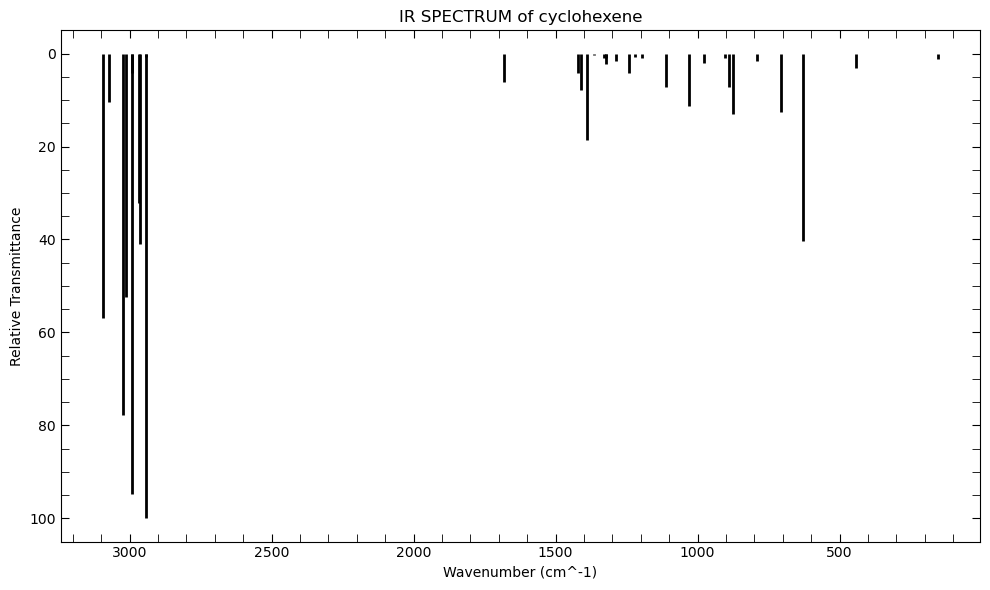
\includegraphics[height=5cm]{Cyclohexene_spectrum.png}
        \caption{Calculated IR spectrum of cyclohexene.}
        \label{fig:cyclohexen_sim}
    \end{subfigure}
    \hfill
    \begin{subfigure}[b]{0.48\textwidth}
        \centering
        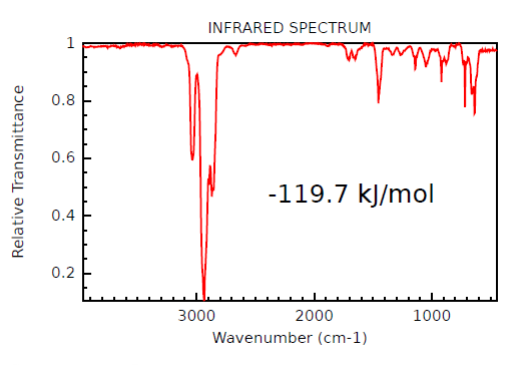
\includegraphics[height=5cm]{Cyclohexene_spectrum_exp.png}
        \caption{Experimental IR spectrum from script.}
        \label{fig:cyclohexan_exx}
    \end{subfigure}
    \caption{Side-by-side comparison of simulated and experimental vibrational data for cyclohexene.}
    \label{fig:cyc}
\end{figure}

In the case of allyl alcohol, the presence of the hydroxyl group and the adjacent vinylic system leads to a spectrum featuring a broad O-H stretching band and a characteristic C=C signal. The correlation between the simulated harmonic frequencies and the experimental reference, specifically the identification of the allylic \ch{CH2}-deformation, is illustrated in \autoref{fig:all}.

\begin{figure}[H]
    \centering
    \begin{subfigure}[b]{0.48\textwidth}
        \centering
        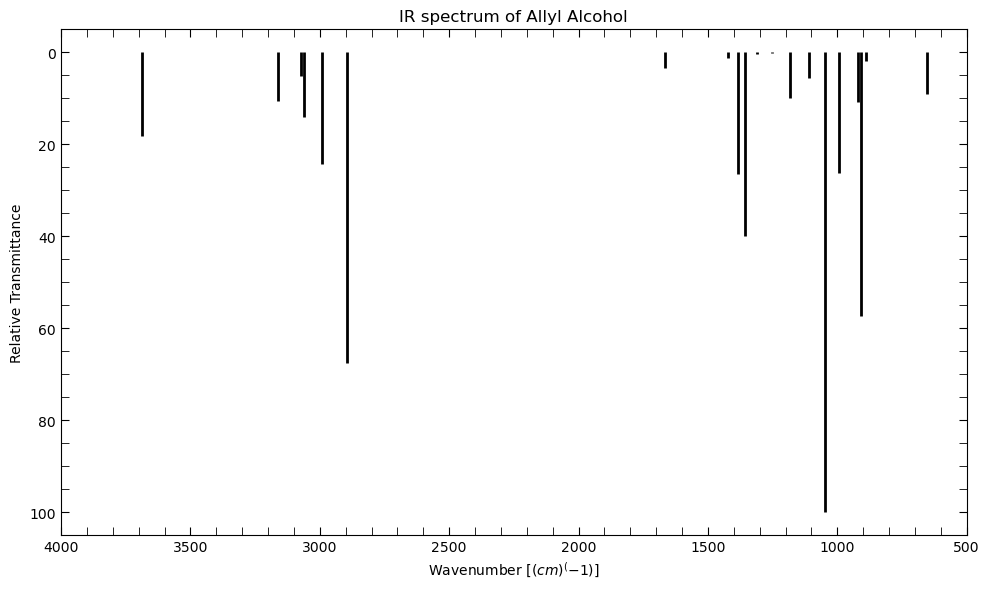
\includegraphics[height=5cm]{allyl_alcohol_spectrum.png}
        \caption{Calculated IR spectrum of allyl alcohol.}
        \label{fig:all_sim}
    \end{subfigure}
    \hfill
    \begin{subfigure}[b]{0.48\textwidth}
        \centering
        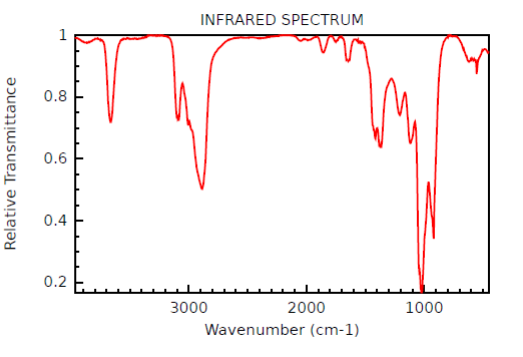
\includegraphics[height=5cm]{allyl_alcohol_spectrum_exp.png}
        \caption{Experimental IR spectrum from script.}
        \label{fig:all_exp}
    \end{subfigure}
    \caption{Side-by-side comparison of simulated and experimental vibrational data for allyl alcohol.}
    \label{fig:all}
\end{figure}

Acrylic acid is identified by the prominent carbonyl (C=O) stretching vibration near \SI{1720}{cm^{-1}}, which is indicative of the conjugated carboxylic acid functional group. \autoref{fig:acr} displays the side-by-side comparison, where the coupling between the C=C and C=O modes provides a unique diagnostic pattern.

\begin{figure}[H]
    \centering
    \begin{subfigure}[b]{0.48\textwidth}
        \centering
        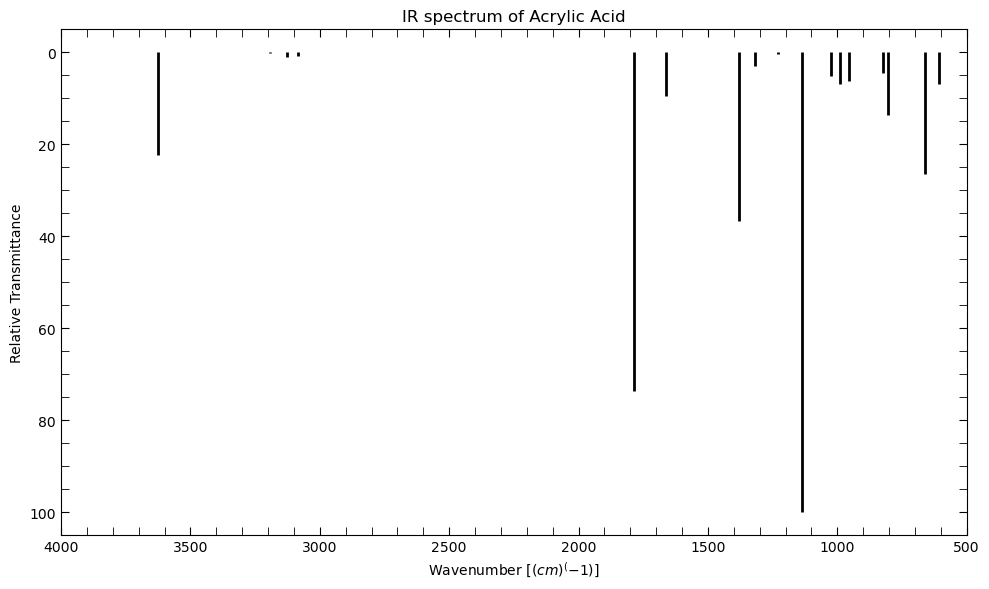
\includegraphics[height=5cm]{acrylic_acid_spectrum.png}
        \caption{Calculated IR spectrum of acrylic acid.}
        \label{fig:acr_sim}
    \end{subfigure}
    \hfill
    \begin{subfigure}[b]{0.48\textwidth}
        \centering
        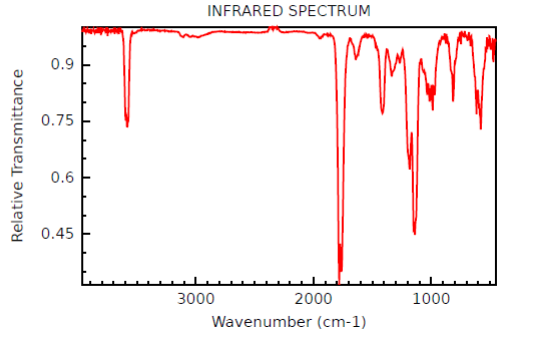
\includegraphics[height=5cm]{acrylic_acid_spectrum_exp.png}
        \caption{Experimental IR spectrum from script.}
        \label{fig:acr_exp}
    \end{subfigure}
    \caption{Side-by-side comparison of simulated and experimental vibrational data for acrylic acid.}
    \label{fig:acr}
\end{figure}

The spectrum of dichloromethane is characterized by the symmetric and antisymmetric C-Cl stretching modes in the fingerprint region between \SI{700}{cm^{-1}} and \SI{800}{cm^{-1}}. The alignment of these theoretically predicted halogen-specific bands with the experimental measurement is depicted in \autoref{fig:comparison_dic}.

\begin{figure}[H]
    \centering
    \begin{subfigure}[b]{0.48\textwidth}
        \centering
        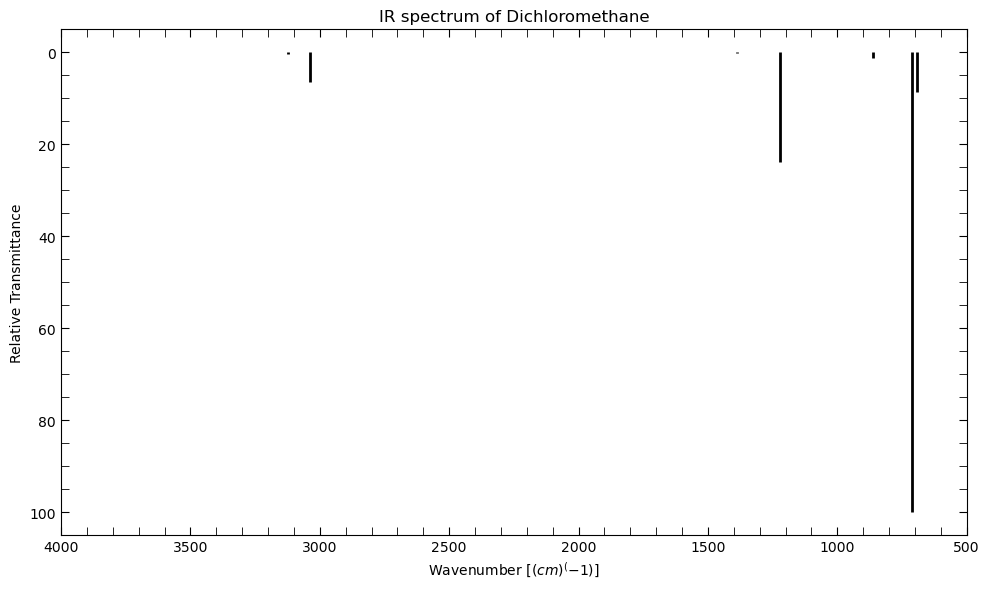
\includegraphics[height=5cm]{dichloromethane.png}
        \caption{Calculated IR spectrum of dichloromethane.}
        \label{fig:dic_sim}
    \end{subfigure}
    \hfill
    \begin{subfigure}[b]{0.48\textwidth}
        \centering
        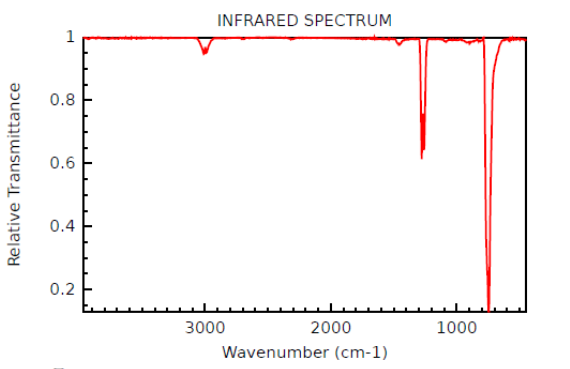
\includegraphics[height=5cm]{dichloromethane_exp.png}
        \caption{Experimental IR spectrum from script.}
        \label{fig:dic_exp}
    \end{subfigure}
    \caption{Side-by-side comparison of simulated and experimental vibrational data for dichloromethane.}
    \label{fig:comparison_dic}
\end{figure}

Finally, salicylic acid exhibits a highly diagnostic spectral pattern due to the intramolecular hydrogen bond between the phenolic O-H and the carboxylic C=O group, which significantly shifts the respective stretching frequencies. The resulting vibrational signatures, including the aromatic ring skeletal vibrations, are compared to the experimental script data in \autoref{fig:sal_exp}.

\begin{figure}[H]
    \centering
    \begin{subfigure}[b]{0.48\textwidth}
        \centering
        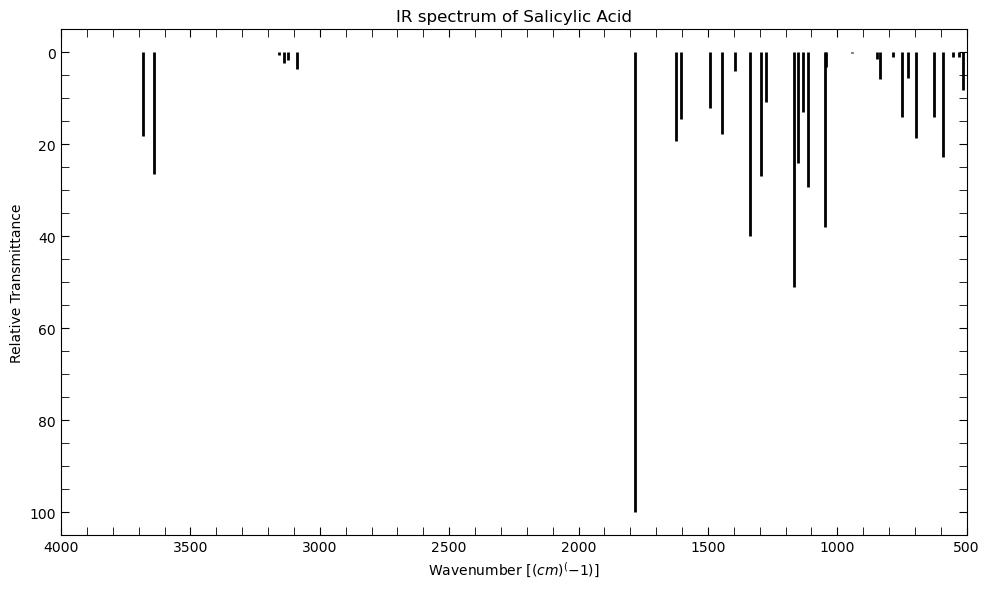
\includegraphics[height=5cm]{salicylic_acid_spectrum.png}
        \caption{Calculated IR spectrum of salicylic acid.}
        \label{fig:sal_sim}
    \end{subfigure}
    \hfill
    \begin{subfigure}[b]{0.48\textwidth}
        \centering
        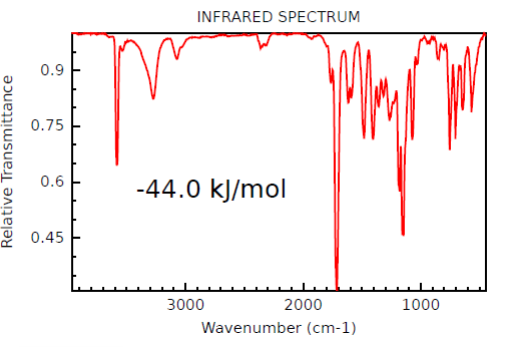
\includegraphics[height=5cm]{salicylic_acid_spectrum_exp.png}
        \caption{Experimental IR spectrum from script.}
        \label{fig:experimental}
    \end{subfigure}
    \caption{Side-by-side comparison of simulated and experimental vibrational data for salicylic acid.}
    \label{fig:sal_exp}
\end{figure}

To further corroborate the structural assignments, the calculated hydration enthalpies were compared with the experimental values provided in the script. For the hydrogenation of cyclohexene to cyclohexane, the experimental enthalpy is reported as $\Delta H_{\text{Hyd}} =$\SI{-119.7}{kJ/mol} (cf. \autoref{fig:cyclohexan_exx}), which shows excellent agreement with the values derived from the geometric optimizations $\Delta H_{\text{Hyd}} =$\SI{-155.353}{kJ/mol}. Similarly, the hydrogenation of acrylic acid yields an experimental hydration enthalpy of $\Delta H_{\text{Hyd}} =$\SI{-44.0}{kJ/mol} (cf. \autoref{fig:acr_exp}), while showing a corresponding theoretical value of $\Delta H_{\text{Hyd}}=$\SI{-59.359}{kJ/mol}. The high degree of consistency between the predicted thermodynamic observables and the experimental benchmarks confirms that the chosen density functional and basis set sufficiently account for the electronic correlation and structural changes associated with these transformations.

The raw computational data yields discrete vibrational frequencies, which do not directly resemble the continuous bands observed in experimental spectra. To simulate a realistic spectral profile, these line spectra are convoluted using a Lorentzian or Gaussian line shape function. This broadening accounts for the finite lifetime of the excited vibrational states and the instrumental resolution of the spectrometer.

The disparity in computational demand between infrared (IR) and Raman spectra arises from the different physical properties and the order of the derivatives involved in their respective simulations. While IR intensities are determined by the change in the molecular dipole moment ($\mu$) during a vibration, Raman intensities depend on the change in the molecular polarizability ($\alpha$). 

From a mathematical perspective, the dipole moment is a first-rank tensor (a vector), whereas the polarizability is a second-rank tensor, represented by a $3 \times 3$ matrix. Consequently, calculating IR intensities requires the second derivative of the total energy with respect to the electric field and the nuclear displacement. In contrast, Raman intensities necessitate the third-order derivative, which significantly increases the complexity of the underlying equations. 

Furthermore, the calculation of polarizability is highly sensitive to the description of the electron cloud's periphery. This requires the use of larger basis sets augmented with diffuse functions to achieve sufficient accuracy, which in turn leads to a substantial increase in memory requirements and CPU time. Additionally, Raman intensities exhibit a greater sensitivity to the numerical integration grid in density functional theory (DFT), requiring finer grids to minimize numerical noise compared to standard IR calculations.

\end{document}